\documentclass[11pt,twocolumn,oneside,openany,headings=optiontotoc,11pt,numbers=noenddot]{article}

\usepackage[a4paper]{geometry}
\usepackage[utf8]{inputenc}
\usepackage[T1]{fontenc}
\usepackage{lmodern}
\usepackage[ngerman]{babel}
\usepackage{ngerman}

\usepackage[onehalfspacing]{setspace}

\usepackage{fancyhdr}
\usepackage{fancybox}

\usepackage{rotating}
\usepackage{varwidth}

%Struktogramme
\usepackage[german,curves]{struktex}

\usepackage{pdflscape}
\usepackage{changepage}
\usepackage{graphicx}
\usepackage[bottom]{footmisc}
\usepackage{transparent}
\usepackage{graphbox}
\graphicspath{
	{Pics/PDFs/}
	{Pics/JPGs/}
	{Pics/PNGs/}
}
\usepackage{caption}
\usepackage{wrapfig}
\usepackage{marginnote}
\usepackage{tabularx}
\usepackage{dashrule}
\usepackage{soulutf8}
\usepackage{hhline}
%arydshln suppresses vertical lines in table
%\usepackage{arydshln}
\usepackage{multirow}
\usepackage{enumerate}
\usepackage[hidelinks]{hyperref}
\usepackage{listings}

\usepackage[table]{xcolor}
\usepackage{array}
\usepackage{enumitem,amssymb,amsmath}
\usepackage{interval}
\usepackage{cancel}
\usepackage{stmaryrd}
\usepackage{wasysym}
\usepackage{polynom}
\usepackage{diagbox}
\usepackage{dashrule}
\usepackage{framed}
\usepackage{mdframed}
\usepackage{karnaugh-map}
\usepackage{pdfpages}

\usepackage{blindtext}

\usepackage{eso-pic}

\usepackage{amssymb}
\usepackage{eurosym}

\usepackage[pages=some]{background}
\pagestyle{headings}
\renewcommand{\headrulewidth}{0.2pt}
\renewcommand{\footrulewidth}{0.2pt}
\newcommand*{\underdownarrow}[2]{\ensuremath{\underset{\overset{\Big\downarrow}{#2}}{#1}}}
\setlength{\fboxsep}{5pt}
\newcommand{\explainBelow}[3]{\underbrace{#1}_{\parbox{\widthof{#3}}{\footnotesize\raggedright #2}}}
\newcommand{\explainAbove}[3]{\overbrace{#1}^{\parbox{\widthof{#3}}{\footnotesize\raggedright #2}}}
\newcommand\footnoteref[1]{\protected@xdef\@thefnmark{\ref{#1}}\@footnotemark}


% Codestyle defined
\definecolor{codegreen}{rgb}{0,0.6,0}
\definecolor{codegray}{rgb}{0.5,0.5,0.5}
\definecolor{codepurple}{rgb}{0.58,0,0.82}
\definecolor{backcolour}{rgb}{0.95,0.95,0.92}
\definecolor{deepgreen}{rgb}{0,0.5,0}
\definecolor{darkblue}{rgb}{0,0,0.65}
\definecolor{mauve}{rgb}{0.40, 0.19,0.28}
\colorlet{exceptioncolour}{yellow!50!red}
\colorlet{commandcolour}{blue!60!black}
\colorlet{numpycolour}{blue!60!green}
\colorlet{specmethodcolour}{violet}

%Neue Spaltendefinition
\newcolumntype{L}[1]{>{\raggedright\let\newline\\\arraybackslash\hspace{0pt}}m{#1}}
\newcolumntype{M}{>{\centering\arraybackslash}X}
\newcommand{\cmnt}[1]{\ignorespaces}
%Textausrichtung ändern
\newcommand\tabrotate[1]{\rotatebox{90}{\raggedright#1\hspace{\tabcolsep}}}

%Intervall-Konfig
\intervalconfig {
	soft open fences
}

%Bash
\lstdefinestyle{BashInputStyle}{
	language=bash,
	basicstyle=\small\sffamily,
	backgroundcolor=\color{backcolour},
	columns=fullflexible,
	backgroundcolor=\color{backcolour},
	breaklines=true,
}
%Java
\lstdefinestyle{JavaInputStyle}{
	language=Java,
	backgroundcolor=\color{backcolour},
	aboveskip=1mm,
	belowskip=1mm,
	showstringspaces=false,
	columns=flexible,
	basicstyle={\footnotesize\ttfamily},
	numberstyle={\tiny},
	numbers=none,
	keywordstyle=\color{purple},,
	commentstyle=\color{deepgreen},
	stringstyle=\color{blue},
	emph={out},
	emphstyle=\color{darkblue},
	emph={[2]rand},
	emphstyle=[2]\color{specmethodcolour},
	breaklines=true,
	breakatwhitespace=true,
	tabsize=2,
}
%Python
\lstdefinestyle{PythonInputStyle}{
	language=Python,
	alsoletter={1234567890},
	aboveskip=1ex,
	basicstyle=\footnotesize,
	breaklines=true,
	breakatwhitespace= true,
	backgroundcolor=\color{backcolour},
	commentstyle=\color{red},
	otherkeywords={\ , \}, \{, \&,\|},
	emph={and,break,class,continue,def,yield,del,elif,else,%
		except,exec,finally,for,from,global,if,import,in,%
		lambda,not,or,pass,print,raise,return,try,while,assert},
	emphstyle=\color{exceptioncolour},
	emph={[2]True,False,None,min},
	emphstyle=[2]\color{specmethodcolour},
	emph={[3]object,type,isinstance,copy,deepcopy,zip,enumerate,reversed,list,len,dict,tuple,xrange,append,execfile,real,imag,reduce,str,repr},
	emphstyle=[3]\color{commandcolour},
	emph={[4]ode, fsolve, sqrt, exp, sin, cos, arccos, pi,  array, norm, solve, dot, arange, , isscalar, max, sum, flatten, shape, reshape, find, any, all, abs, plot, linspace, legend, quad, polyval,polyfit, hstack, concatenate,vstack,column_stack,empty,zeros,ones,rand,vander,grid,pcolor,eig,eigs,eigvals,svd,qr,tan,det,logspace,roll,mean,cumsum,cumprod,diff,vectorize,lstsq,cla,eye,xlabel,ylabel,squeeze},
	emphstyle=[4]\color{numpycolour},
	emph={[5]__init__,__add__,__mul__,__div__,__sub__,__call__,__getitem__,__setitem__,__eq__,__ne__,__nonzero__,__rmul__,__radd__,__repr__,__str__,__get__,__truediv__,__pow__,__name__,__future__,__all__},
	emphstyle=[5]\color{specmethodcolour},
	emph={[6]assert,range,yield},
	emphstyle=[6]\color{specmethodcolour}\bfseries,
	emph={[7]Exception,NameError,IndexError,SyntaxError,TypeError,ValueError,OverflowError,ZeroDivisionError,KeyboardInterrupt},
	emphstyle=[7]\color{specmethodcolour}\bfseries,
	emph={[8]taster,send,sendMail,capture,check,noMsg,go,move,switch,humTem,ventilate,buzz},
	emphstyle=[8]\color{blue},
	keywordstyle=\color{blue}\bfseries,
	rulecolor=\color{black!40},
	showstringspaces=false,
	stringstyle=\color{deepgreen}
}

\lstset{literate=%
	{Ö}{{\"O}}1
	{Ä}{{\"A}}1
	{Ü}{{\"U}}1
	{ß}{{\ss}}1
	{ü}{{\"u}}1
	{ä}{{\"a}}1
	{ö}{{\"o}}1
}

% Neue Klassenarbeits-Umgebung
\newenvironment{worksheet}[3]
% Begin-Bereich
{
	\newpage
	\sffamily
	\setcounter{page}{1}
	\ClearShipoutPicture
	\AddToShipoutPicture{
		\put(55,761){{
				\mbox{\parbox{385\unitlength}{\tiny \color{codegray}BBS I Mainz, #1 \newline #2
						\newline #3
					}
				}
			}
		}
		\put(455,761){{
				\mbox{\hspace{0.3cm}
\includegraphics[width=0.2\textwidth]{../../logo.pdf}}
			}
		}
	}
}
% End-Bereich
{
	\clearpage
	\ClearShipoutPicture
}

\setlength{\columnsep}{3em}
\setlength{\columnseprule}{0.5pt}

\geometry{left=2.50cm,right=2.50cm,top=3.00cm,bottom=1.00cm,includeheadfoot}
\pagenumbering{gobble}
\pagestyle{empty}

\begin{document}
	\begin{worksheet}{HBF IT 17A}{Grundstufe}{Lernbaustein 3 - LB 2: Differenzialrechnung - Ableitungsfunktion}
		\section{Was sagt uns die Ableitungsfunktion?}
		Zu jeder Stelle eines Graphen können wir eine Steigung \(m\) z.B. mittels dem Differenzialquotienten ermitteln. 
		Indem wir jeder Stelle \(x\) ihre Steigung \(m\) zuordnen, erhalten wir eine neue Funktion \(f'\), die \textbf{Ableitungsfunktion von \(\mathbf{f}\)}.
		\subsection*{Beispiel 1}
		Betrachten wir die nachfolgende Funktion \(f(x)\) und deren Ableitungsfunktion \(f'(x)\).
		\begin{align*}
			f(x) = \frac{1}{2}x^2+5x\\
			f'(x) = x + 5
		\end{align*}
		In der nachstehenden Tabelle sind für sieben Stellen \textit{x} die zugehörigen Steigungen
		\begin{center}
			\begin{tabular}{c|c|c|c|c|c|c|c}
				\textit{x} & -10 & -8 & -6 & -4 & -2 & 0 & 2\\
				\hline
				\(f'(x)\) & -5 & -3 & -1 & 1 & 3 & 5 & 7
			\end{tabular}
		\end{center}
		Das obere Koordinatensystem zeigt den Graphen der Funktion \(f\) mit \(f(x) = \frac{1}{2}x^2+5x\).\\
		\par\noindent
		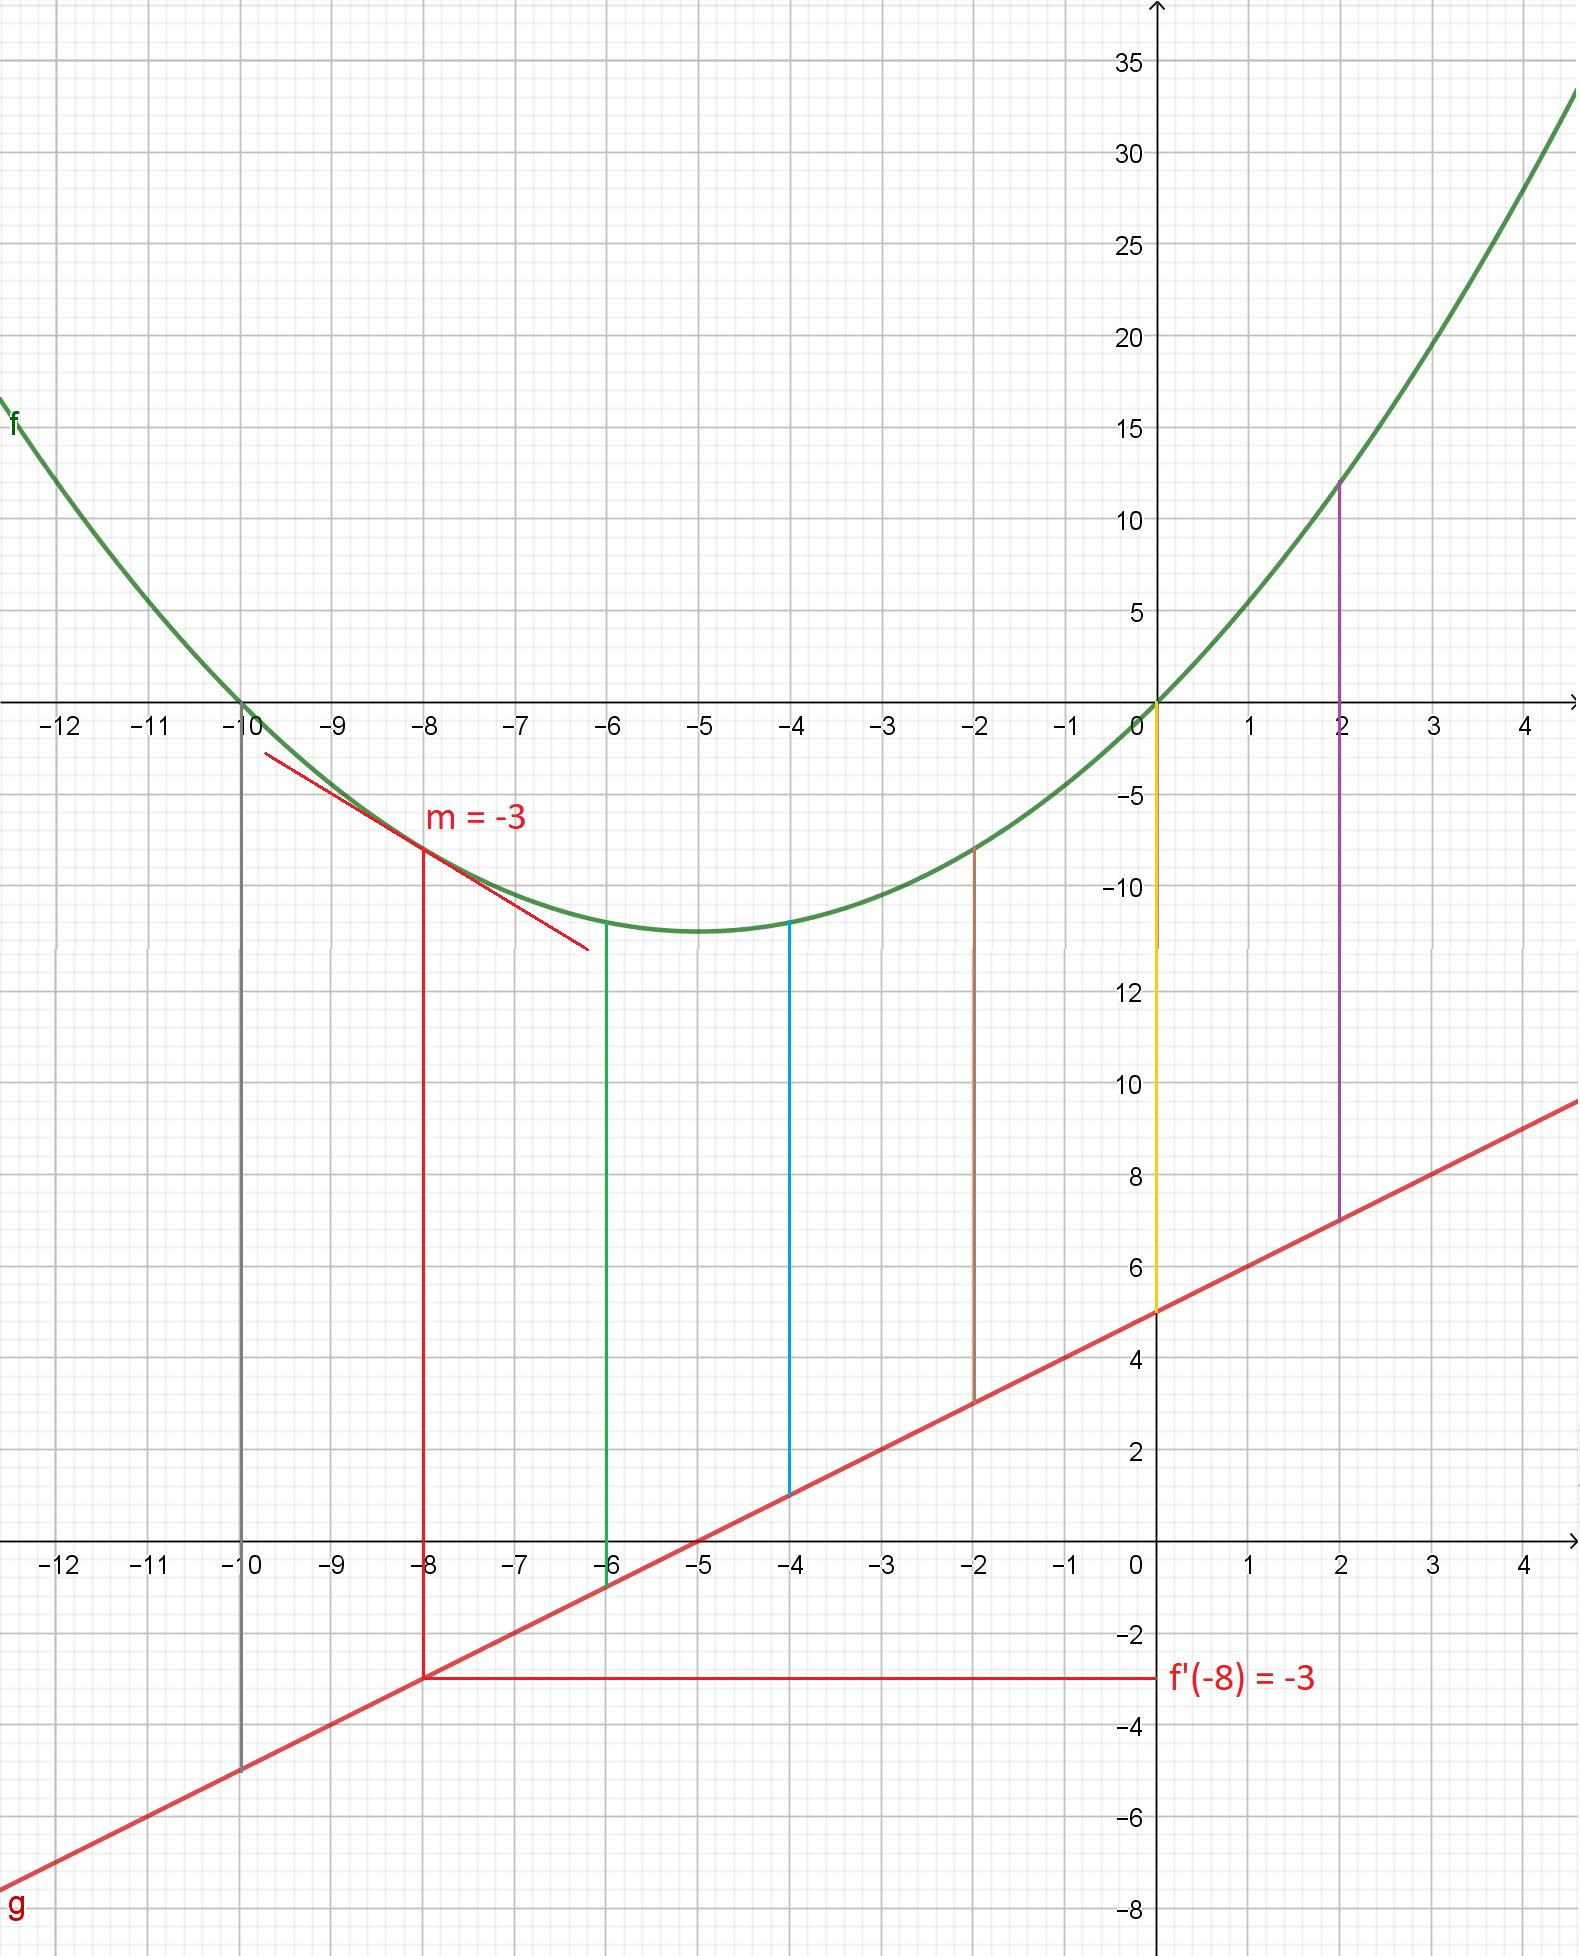
\includegraphics[scale=0.26]{Bilder/ff'.png}\\
		Der Zusammenhang ist an der Stelle \(x=-8\) verdeutlicht: Im ersten Koordinatensystem sehen wir, dass der Graph von \(f\) an der Stelle \(x=-8\) die Steigung \(m=-3\) hat.\\
		Im zweiten Koordinatensystem ist der Graph der Ableitungsfunktion \(f'\) mit \(f'(x)= x+5\) dargestellt. Hier wird der Stelle \(x=-8\) der \textit{y}-Wert \(-3\) zugeordnet. Der \textit{y}-wert entspricht also der Steigung an der untersuchten Stelle.
		\subsection*{Interessante Stellen}
		Das Steigungsverhalten eines Funktionsgraphen mithilfe von Tangenten in einzelnen Punkten zu beschreiben, ist ziemlich aufwändig. Meist ist es ausreichend, das Steigungsverhalten für bestimmte Abschnitte des Funktionsgraphen zu untersuchen.\\
		Betrachten wir den nachstehenden Graphen einer ganzrationalen Funktion 4. Grades und unterteilen die
		sen nach steigenden und fallenden Abschnitten.\\
		\par\noindent
		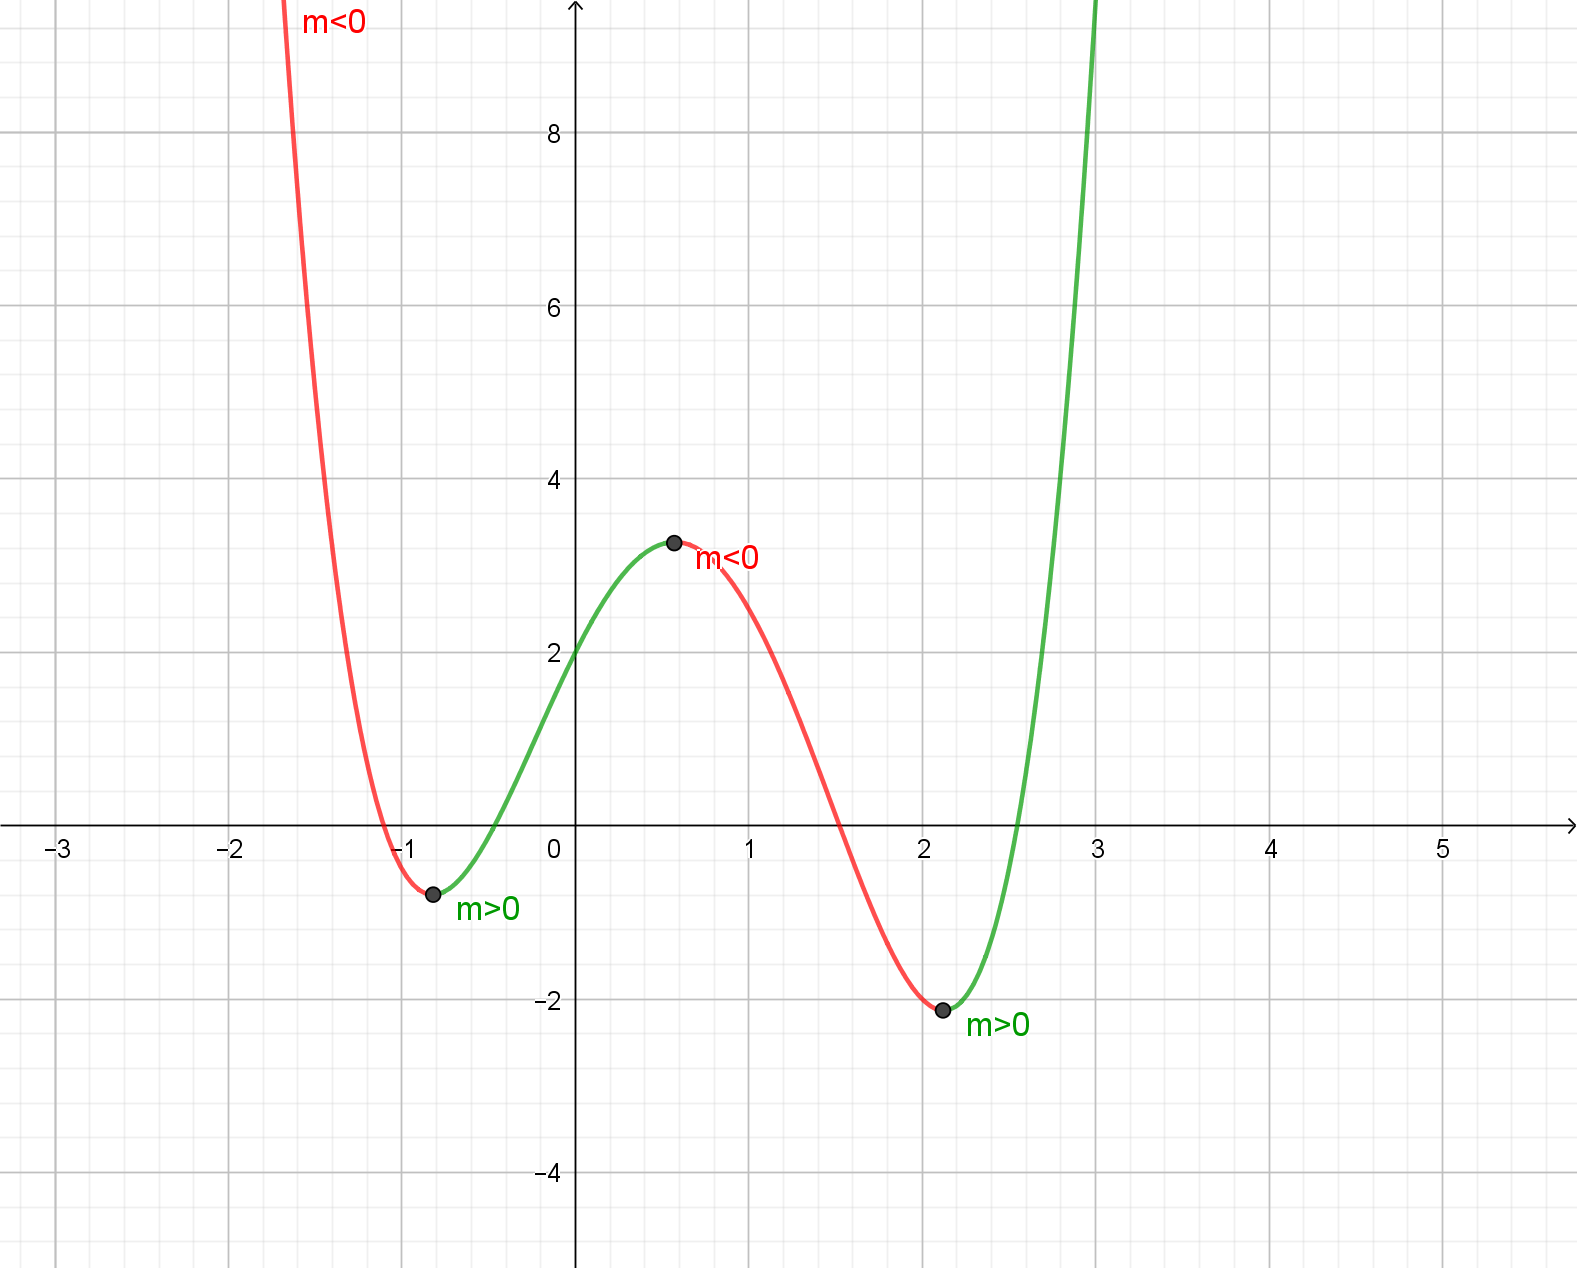
\includegraphics[scale=0.26]{Bilder/fAbsch.png}\\
		Innerhalb der steigenden Abschnitten ergeben sich Tangenten mit positiver Steigung (\color{codegreen}{m>0}\normalcolor). Hier hat der Graph positive Steigungswerte. Entsprechend gilt für die fallenden Abschnitte des Graphen: Hier sind die Steigungswerte negativ (\color{red}{m<0}\normalcolor). An den Übergängen erhalten wir jeweils eine waagrechte Tangente, also \color{blue}{m=0}\normalcolor.\\
		Um den Steigungsgraphen zu skizzieren, markieren wir zunächst auf der \textit{x}-Achse die Stellen, an denen der Graph von \(f\) die Steigung 0 hat. Da die Funktionswerte des Steigungsgraphen den Steigungswerten des Graphen von \(f\) entsprechen, hat der Steigungsgraph an den markierten Stellen jeweils den \textit{y}-Wert 0. Die markierten Punkte sind also schon Punkte auf unserem Steigungsgraphen.\\
		\par\bigskip\noindent
		Haben wir die Punkte eingezeichnet, überlegen wir, wie der zugehörige Steigungsgraph zwischen den Markierten Punkten aussieht. Bis zu unserem ersten Punkt fällt der Graph von \(f\), d.h. die Steigungswerte sind negativ. Der Steigungsgraph verläuft also \color{red}{unterhalb der \(x\)-Achse}\normalcolor.\\
		Zwischen dem ersten und zweiten Punkt steigt der Graph von \(f\), die Steigungswerte sind also positiv. Der dazugehörige Graph verläuft also \color{codegreen}{oberhalb der \(x\)-Achse}\normalcolor.\\
		Im nächsten Abschnitt fällt der Graph von \(f\) wieder, der Steigungsgraph befindet sich also \color{red}{unterhalb der \(x\)-Achse}\normalcolor.\\
		Der Graph rechts vom letzten Punkt steigt schließlich nur noch, d.h. der sazugehörige Steigungsgraph muss \color{codegreen}{oberhalb der \(x\)-Achse }\normalcolor liegen.\\
		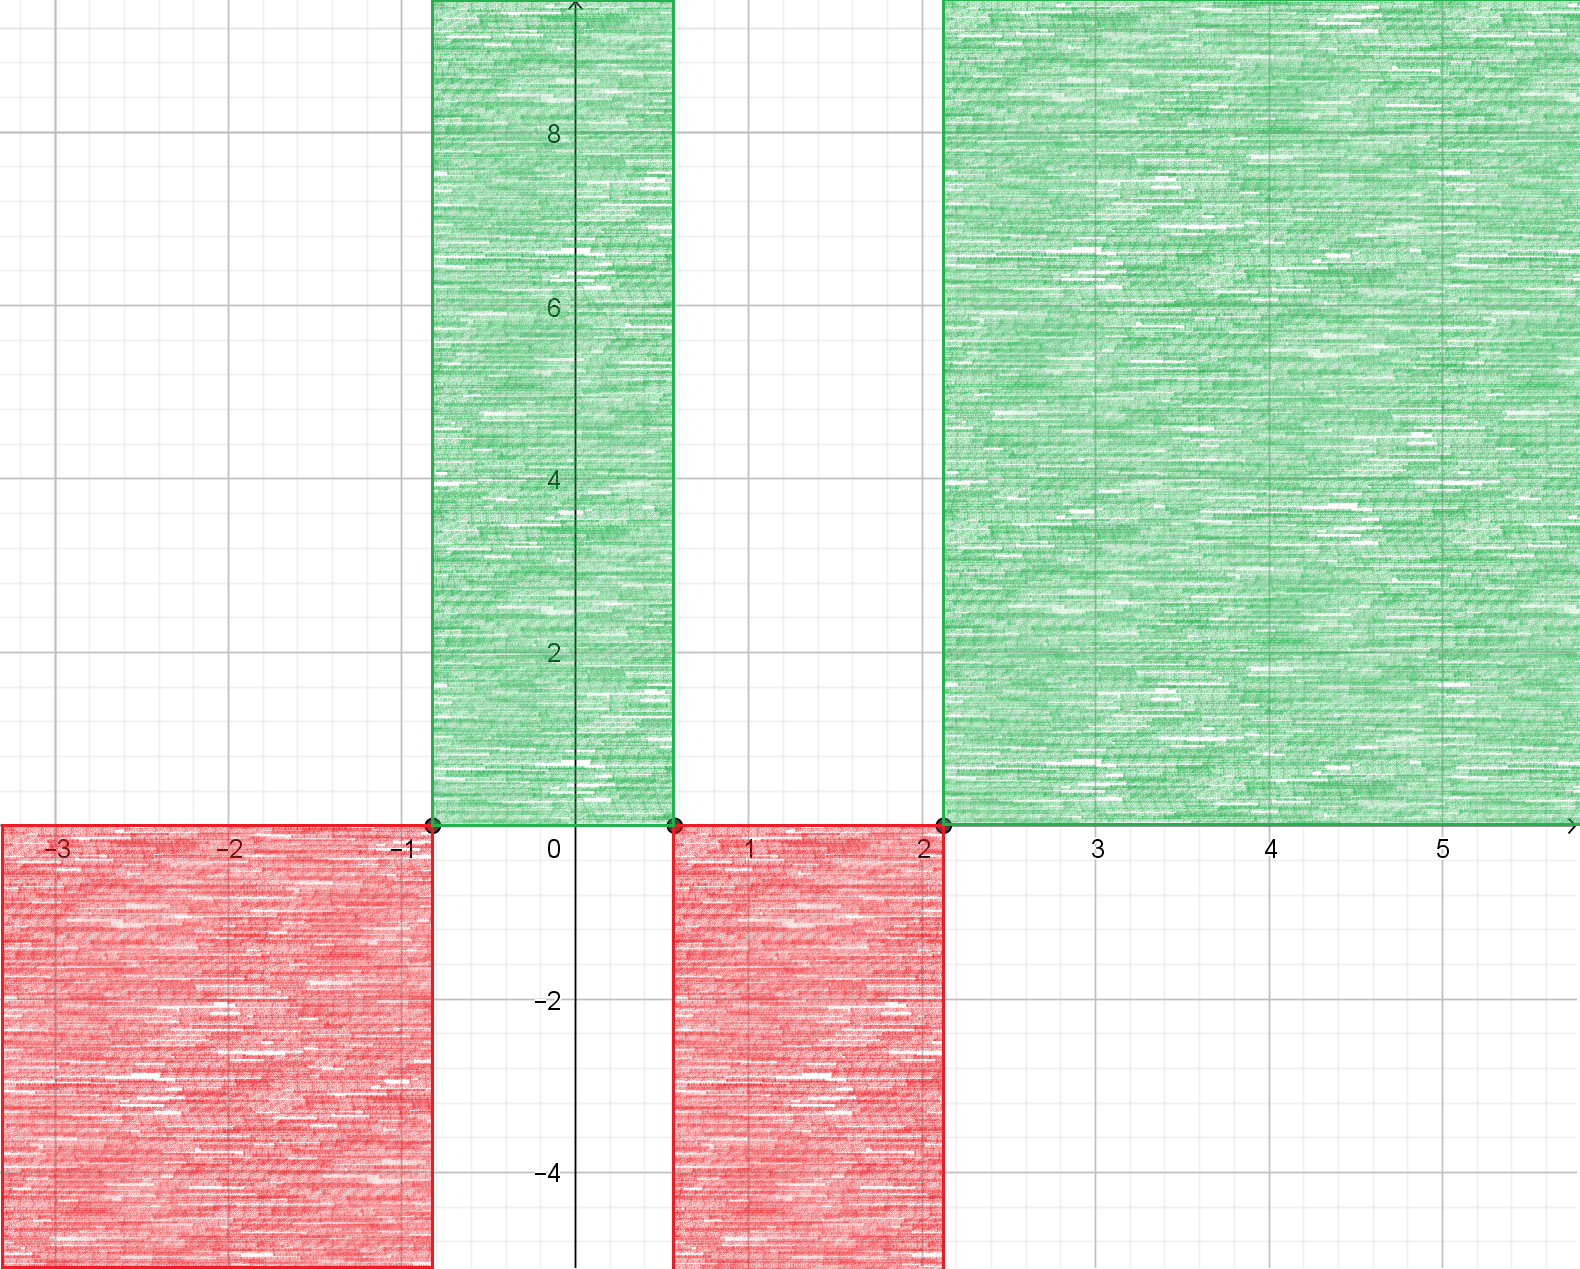
\includegraphics[scale=0.25]{Bilder/fGef.png}\\
		\par\noindent
		Wir wissen also nun, wo der Steigungsgraph oberhalb bzw. unterhalb er \(x\)-Achse liegt und an welchen Stellen er die \(x\)-Achse schneidet.\\
		Wir können ihn mit diesem Wissen also schon relativ genau zeichnen.\\
		\par\noindent
		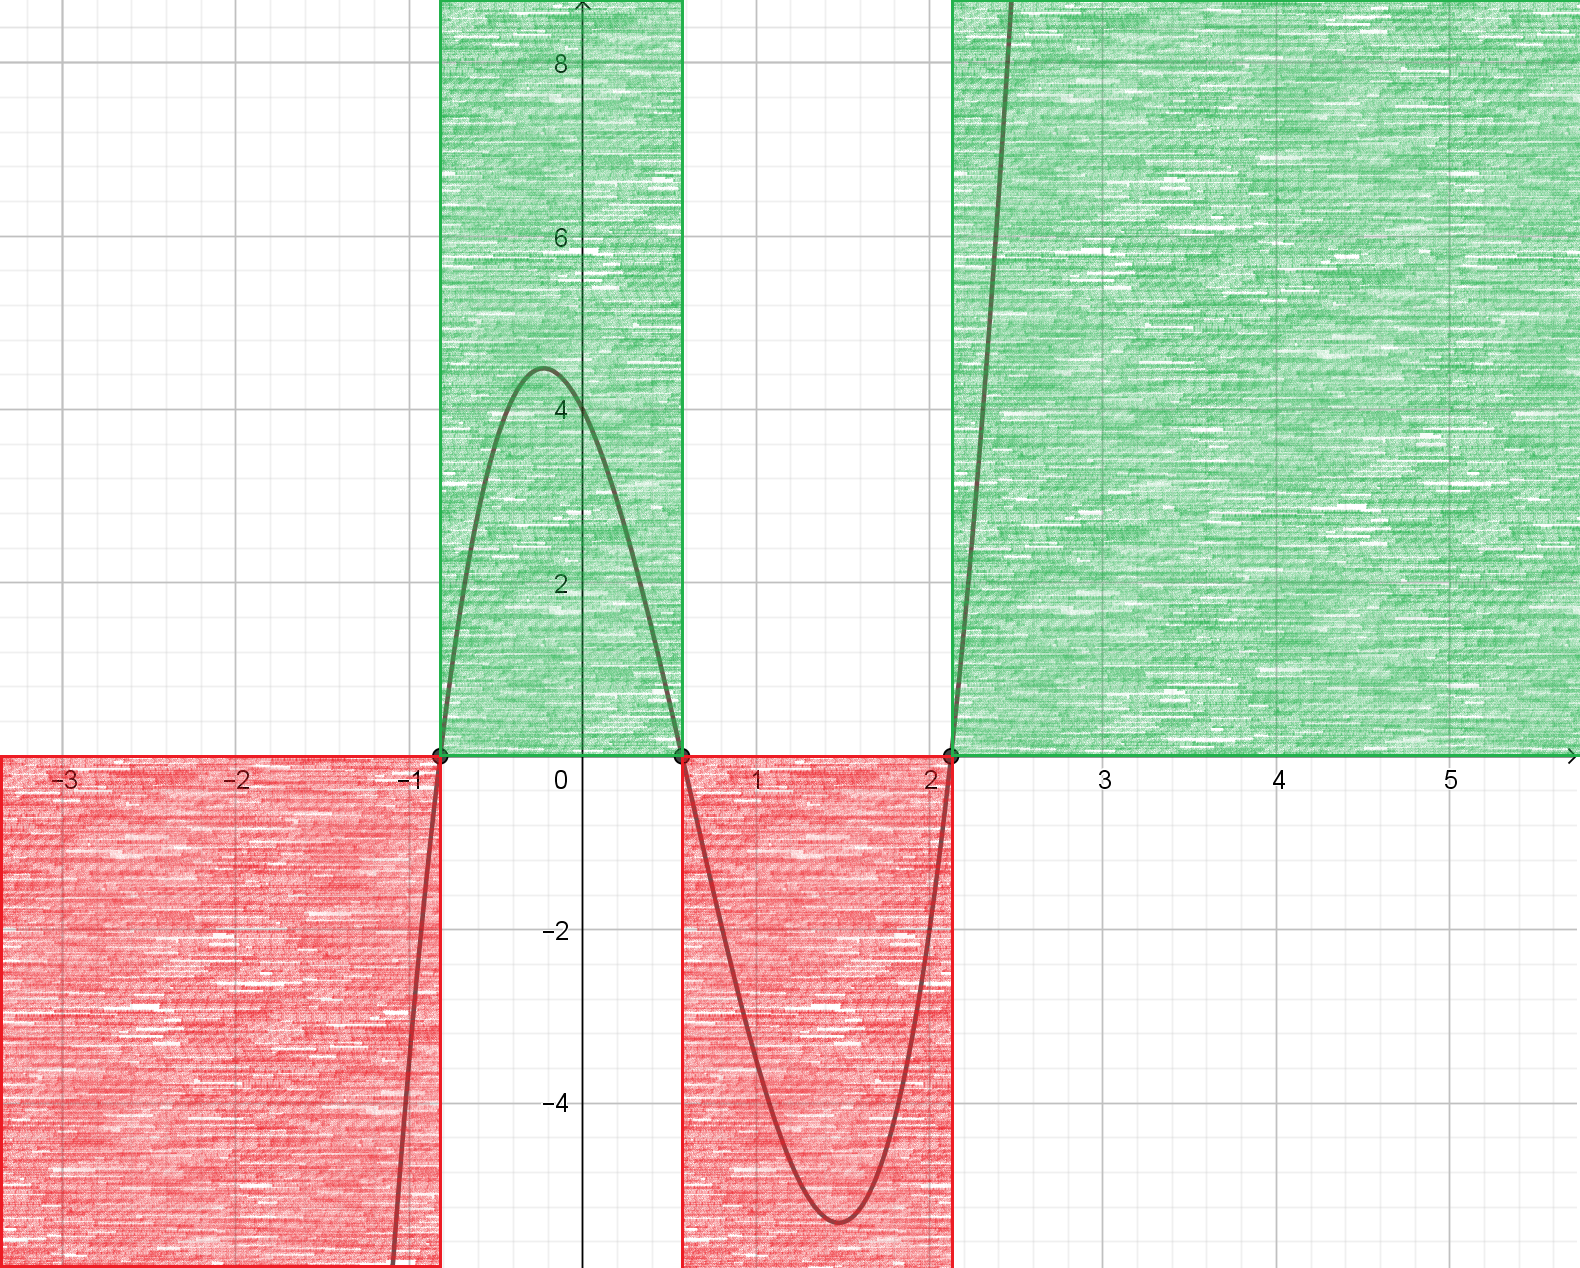
\includegraphics[scale=0.25]{Bilder/f'Absch.png}
		\subsection{Zusammenfassung}
		Betrachten wir eine Funktion \(f(x)\) und den dazugehörigen Funktionsgraphen, so gibt es verschiedene Stellen, die interessant sind.
		\begin{framed}
			\noindent
			Zunächst suchen wir die Stellen, an denen die Steigung \(m\) des Funktionsgraphen von \(f(x)\) 0 ist. Dies ist genau dann der Fall, wenn die Ableitungsfunktion \(f'(x)\) den Wert 0 annimmt. Also wenn gilt: \[f'(x) = 0\]\\
			\tiny{\color{codegray}Vorgehen}\normalsize
			\begin{itemize}
				\item[-] Bestimme zunächst die Ableitungsfunktion \(f'(x)\)
				\item[-] Berechne anschließend die Nullstellen der Ableitungsfunktion \(f'(x)\)
			\end{itemize}
			Die so ermittelten \(x\)-Werte sind die Stellen, an denen der Funktionsgraph von \(f(x)\) seinen Verlauf ändert.
		\end{framed}
		
	\end{worksheet}
\end{document}